\documentclass{./../div_teaching_slides}
\usepackage{setspace}

\begin{document}
\title{ECON 340 \\ Economic Research Methods}
\author{Div Bhagia \\\vspace{1.75em}
Lecture 2 \\\vspace{0.25em} \small Empirical Distribution \& Measures of Central Tendency}
\date{}

\begin{frame}[noframenumbering, plain]
\maketitle
\end{frame}


%%%%%%%%%%%%%%%%%%%%
\begin{frame}{Describing Data}
A dataset is a collection of variables. Each variable contains multiple observations of the same measurement. \\~\\
\textit{Types of variables:} \\
\begin{witemize}
\item \textit{Categorical}: gender, race, education (\textit{binary}: two categories) 
\item \textit{Continuous}: income, age, GPA \\~\\
\end{witemize}
\textit{How do we summarize the information contained in a variable?} \\~\\
\end{frame}

\begin{frame}{The Empirical Distribution}
How often do different values occur? \\~\\
For categorical variables:
$$ f_k = \frac{n_k}{n}= \frac{\text{observations in category $k$}}{\text{total observations}} $$ \\~\\
$f_k$ captures the relative frequency of outcome $k$. 
\end{frame}

\begin{frame}{Frequency Distribution Table}
\setstretch{1.3}
% latex table generated in R 4.2.1 by xtable 1.8-4 package
% Thu Aug 24 10:46:35 2023
\begin{table}[ht]
\centering
\begin{tabular}{lll}
 Education & Count & Percent \\ 
  \hline
$<$ HS & 1540 &  6.39 \\ 
  HS Grad & 7388 & 30.64 \\ 
  Some College & 5595 & 23.20 \\ 
  4 Year College & 5979 & 24.80 \\ 
  $>$ College & 3611 & 14.98 \\ 
   \hline
Total & 24113 & 100 \\ 
  \end{tabular}
\end{table}

\end{frame}

\begin{frame}{Frequency Distribution Table}
\setstretch{1.3}
% latex table generated in R 4.2.1 by xtable 1.8-4 package
% Thu Aug 24 10:46:35 2023
\begin{table}[ht]
\centering
\begin{tabular}{llll}
 Education & Count & Percent & Cumulative \\ 
  \hline
$<$ HS & 1540 &  6.39 &   6.39 \\ 
  HS Grad & 7388 & 30.64 &  37.03 \\ 
  Some College & 5595 & 23.20 &  60.23 \\ 
  4 Year College & 5979 & 24.80 &  85.02 \\ 
  $>$ College & 3611 & 14.98 & 100.00 \\ 
   \hline
Total & 24113 & 100 &  \\ 
  \end{tabular}
\end{table}

\end{frame}

\begin{frame}{Histogram: Education}
\vspace{-0.5em}
\centering
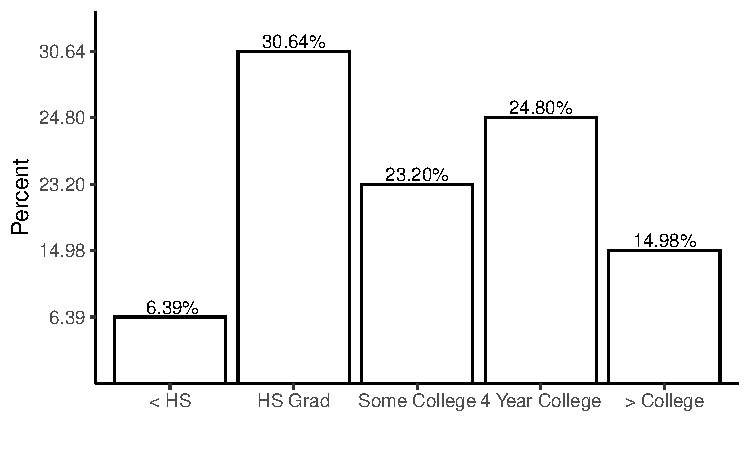
\includegraphics{./../../Output/educ_hist.pdf}
\end{frame}

\begin{frame}{The Empirical Distribution}
What about continuous variables? \pause \\~\\
How often do different values occur in a particular interval? \\~\\
$$ f_k = \frac{\text{observations in \textit{interval} $k$}}{\text{total observations}} $$
\end{frame}

\begin{frame}{Histogram: Household Income}
\centering
\vspace{-0.9em}
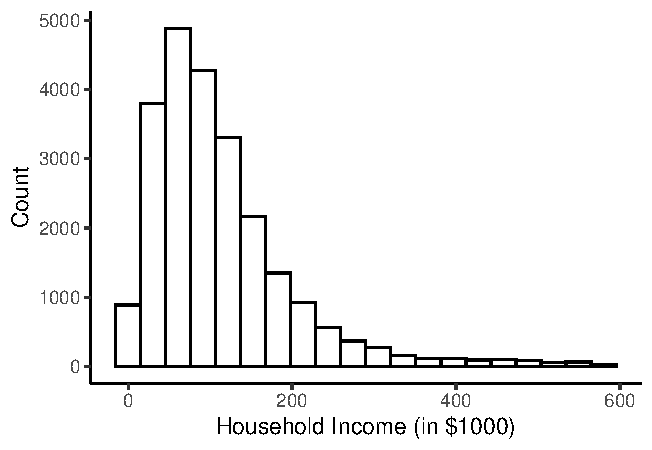
\includegraphics{./../../Output/hhi_hist.pdf} \\
\scriptsize Source: American Community Survey (ACS) 2019
\end{frame}

%%%%%%%%%%%%%%%%%%%%
\begin{frame}{Measures of Central Tendency}
\begin{itemize}
\item[] \underline{\textbf{Mean}}: is the average value \\~\\ 
\item[] \underline{\textbf{Median}}: is the middle value \\~\\
\item[] \underline{\textbf{Mode}}: is the number that is repeated more often than any other \\~\\
\end{itemize} 
\underline{Example}: 5, 5, 10, 10, 10, 10, 20 
\end{frame}

%%%%%%%%%%%%%%%%%%%%
\begin{frame}{Mean}
\vspace{1em}
To calculate the mean:
$$ \bar{X} = \frac{\text{sum of all observations}}{\text{number of observations}} = \frac{1}{n}\sum_{i=1}^n X_i $$ \\~\\
Use $\bar{X}$ to denote the sample mean and $\mu$ to denote the population mean. 
\end{frame}


\begin{frame}{Mean vs Median}
\centering
\vspace{-0.75em}
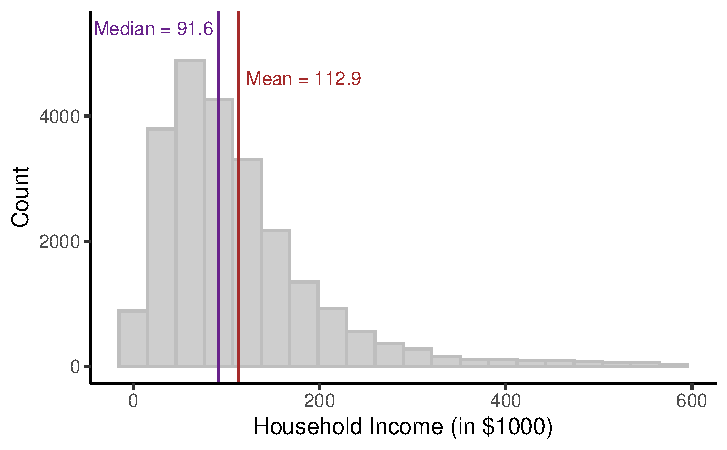
\includegraphics{./../../Output/hhi_hist_mean_med.pdf} \\
\scriptsize Source: American Community Survey (ACS) 2019
\end{frame}

\begin{frame}{Mean vs Median}
\begin{witemize}
\item Mean household income: \$112,900
\item Median household income: \$91,600 \\~\\
\end{witemize} 
Why are mean earnings higher than the median?
\end{frame}

\begin{frame}{Percentiles}
The \textbf{$P^{th}$ percentile} is a value such that $P$\% of observations are at or below that number. \\~\\
\begin{itemize}
\item [] 25th percentile a.k.a 1st quartile
\item [] 75th percentile a.k.a 3rd quartile \\~\\
\end{itemize}
\textit{What is the 50th percentile called?} \\~\\
\end{frame}

\begin{frame}{More about Mean}
\vspace{0.5em}
\begin{itemize}
\item $\sum_{i=1}^n X_i = n \bar{X}$ \\~\\ \pause
\item Deviations from the mean are always zero
$$ \sum_{i=1}^n (X_i-\bar{X}) =  \sum_{i=1}^n X_i - n \bar{X} = n \bar{X}- n \bar{X}=0 $$ \pause
\item We can always write
$$ \bar{X} = \frac {\sum_{i=1}^n X_i}{n} = \frac{1}{n}\sum_{i=1}^n X_i = \sum_{i=1}^n \frac{X_i}{n} $$
\end{itemize}
\end{frame}

\begin{frame}[t]{An easier way to calculate mean}
\vspace{-0.5em}
\begin{witemize}
  \item If data is grouped, we can use the frequency distribution table to calculate the mean: \\ 
$$ \bar{X} = \frac{\sum_{k=1}^K n_k X_k}{n} = \sum_{k=1}^K f_k X_k  $$ \\~\\ \vspace{-0.5em}
  \item Previous example: 5, 5, 10, 10, 10, 10, 20 \\
\end{witemize}
\begin{center}
\begin{tabular}{|c|c|p{1cm}|p{2cm}|}
\hline
$X_k$ & \hspace{0.5em} $n_k$ & \hspace{0.2em} $f_k$ & \hspace{0.2em} $X_k f_k$ \\
\hline
 5 & 2 & & \\
 \hline
10 &  4 & & \\
\hline
20 &  1 & & \\
\hline
Total & 7  & &  \\
\hline 
\end{tabular} 
\end{center}
\vspace{0.5em}

\end{frame}

\begin{frame}{Weighted Mean}
The weighted mean of a set of data is 
$$ \bar{X} = \frac{\sum_{i=1}^nw_i X_i}{\sum_{i=1}^n w_i} $$
where $w_i$ is the weight of the $i^{th}$ observation. \\~\\

Why might we want to use a weighted mean?
\end{frame}

\begin{frame}{2016 Election Predictions}
\centering
 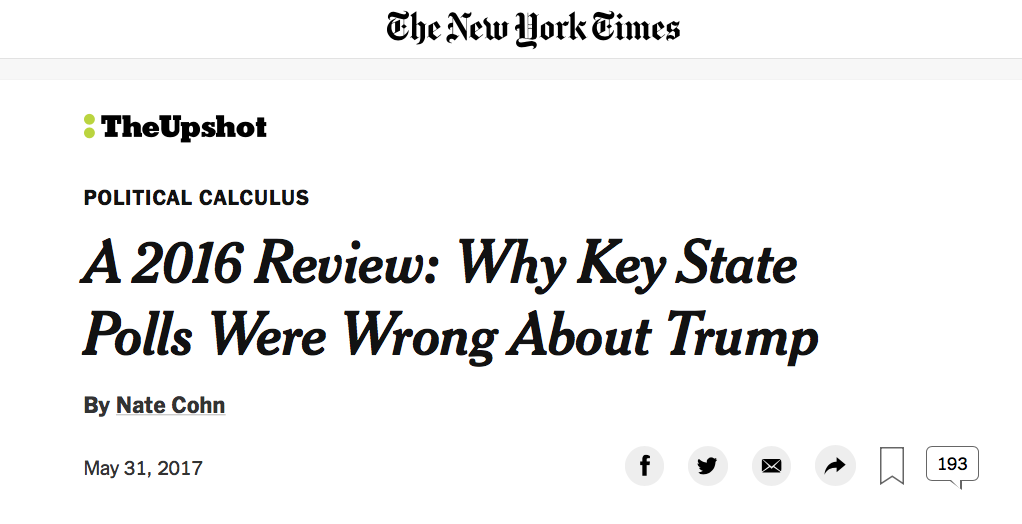
\includegraphics[scale=0.14]{nyt2.png} \\
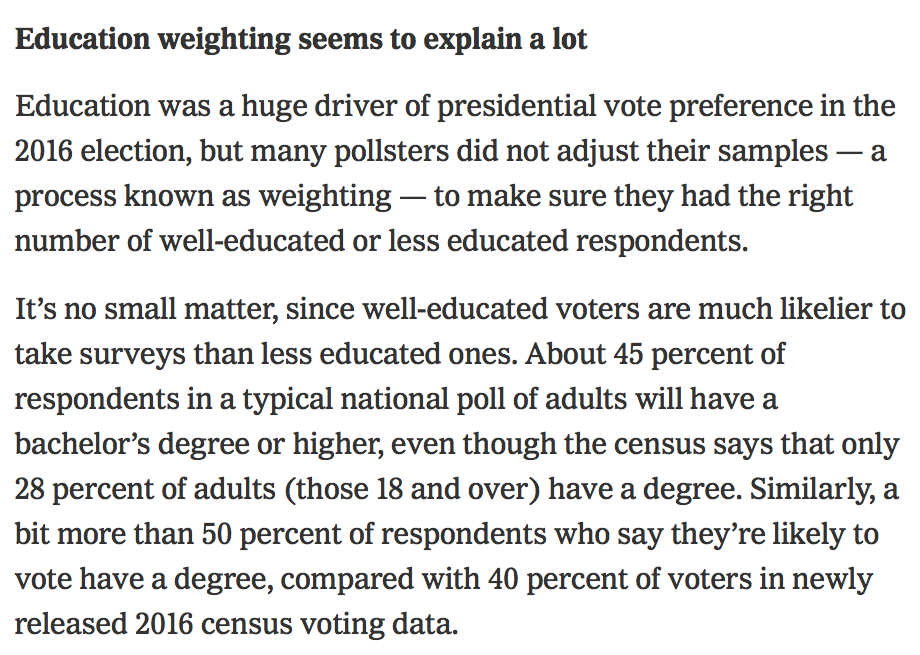
\includegraphics[scale=0.19]{nyt.png} \\
\end{frame}


\begin{frame}{Things to do next}
\begin{witemize}
\item Review this week's material; handouts and reading (NYT article) on Canvas
\item You may be asked to summarize what you got out of the reading in the next class
\item Let me know the members of your research group by end of the day next Thursday
\vspace{0.5em}
\begin{witemize}
\normalsize
\item You can self-sign up on Canvas by going to People and then clicking on the Research Project Group tab
\item Or just send me an email
\end{witemize}
\end{witemize}
\end{frame}

\end{document}